\documentclass[12pt]{article}

%%%%%%%%%%%%%%%%%%%%%%%%%%%%
%%%%%%%%%%%%%%%%%%%%%%%%%%%%
% Load in packages
\usepackage{amsmath}
\usepackage{amssymb}
\usepackage{hyperref}
\usepackage{graphicx}
\usepackage[top=1in, bottom=1in, left=1in, right=1in]{geometry}

%%%%%%%%%%%%%%%%%%%%%%%%%%%%
%%%%%%%%%%%%%%%%%%%%%%%%%%%%

\begin{document}

\begin{center}
\Large Chapter 3 Practice Problems Solutions

\medskip

\normalsize Elements of Microeconomics (discussion section 4)

\medskip

\small John Green
\end{center}

\medskip

\section*{Question 1}
Stu's Steakhouse and Sandie's Salads are two restaurants which serve salads and steaks. Given 1000 minutes of labor time, they can produce the following amounts of each dish:

\begin{table}[h]
  \centering
  \begin{tabular}{|c|c|c|}
    \hline
    \textbf{Restaurant} & \textbf{Steaks} & \textbf{Salads} \\
    \hline
    \textbf{Stu's Steakhouse} & 100 & 20 \\
    \hline
    \textbf{Sandie's Salads} & 200 & 100 \\
    \hline
  \end{tabular}
  \caption{Stu vs. Sandie}
\end{table}


\subsection*{Part A}

What is their cost, in minutes, to produce steak and salads?

\medskip

\textbf{Answer:}

\begin{table}[h]
  \centering
  \begin{tabular}{|c|c|c|}
    \hline
    \textbf{Restaurant} & \textbf{Minutes per steak} & \textbf{Minutes per salad} \\
    \hline
    \textbf{Stu's Steakhouse} & 10 & 50 \\
    \hline
    \textbf{Sandie's Salads} & 5 & 10 \\
    \hline
  \end{tabular}
  \caption{Stu vs. Sandie}
\end{table}

\medskip

\subsection*{Part B}
Assume that there is a constant transferability of productive resources from one dish to the other:
\begin{enumerate}
    \item Draw the production possibility frontiers for the two restaurants.
    \item Who has the absolute advantage in producing steaks?
    \item Who has the absolute advantage in producing salads?
\end{enumerate}

\textbf{Answer:}

\textbf{1.} The two PPFs should look like figures \ref{fig:stuPPF} and \ref{fig:sandiePPF}.

\begin{figure}
    \centering
    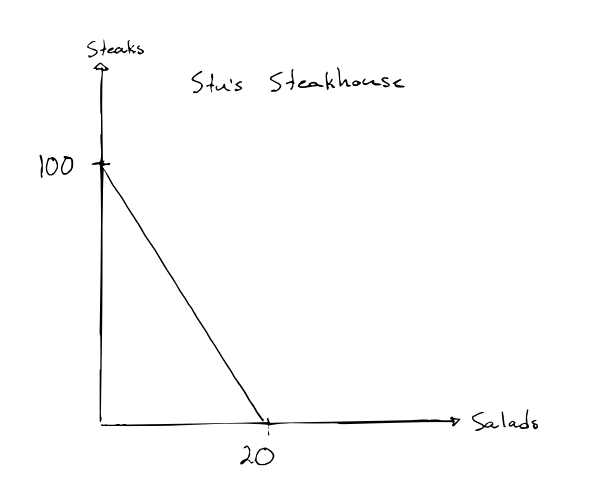
\includegraphics[width=.6\textwidth]{stuPPF.png}
    \caption{PPF of Stu's Steakhouse}
    \label{fig:stuPPF}
\end{figure}

\begin{figure}
    \centering
    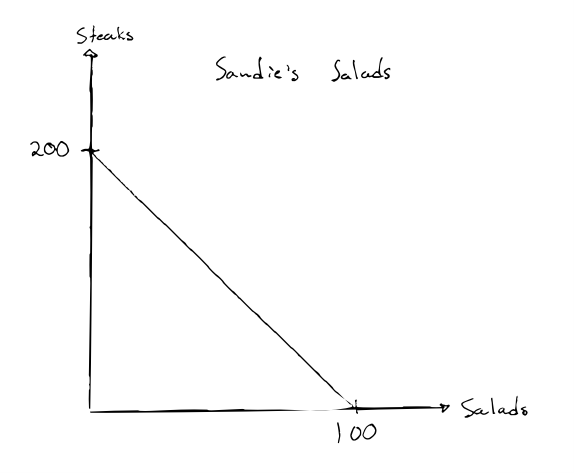
\includegraphics[width=.6\textwidth]{sandiePPF.png}
    \caption{PPF of Sandie's Salads}
    \label{fig:sandiePPF}
\end{figure}

\textbf{2. and 3.} Of course Sandie has the absolute advantage in both dishes.

\subsection*{Part C}
Let's think about the opportunity cost of each firm for each dish:
\begin{enumerate}
    \item What are the slopes of the two PPFs?
    \item What is Stu's opportunity cost for producing steaks and salads?
    \item What is Sandie's opportunity cost for producing steaks and salads?
\end{enumerate}

\textbf{Answer:}

\textbf{1.} The slope of Stu's PPF is $-5$ and the slope of Sandie's PPF is $-2$.

\textbf{2.} Stu faces an opportunity cost to produce 1 steak of $\frac{1}{5}$ of a salad. The opportunity cost to produce 1 salad, on the other hand, is 5 steaks.

\textbf{3.} Sandie faces an opportunity cost to produce 1 steak of $\frac{1}{2}$ of a salad, and the opportunity cost to produce 1 salad of 2 steaks.

\medskip

\subsection*{Part D}

\begin{enumerate}
    \item Can a firm have an absolute advantage in both goods?
    \item Can a firm have a comparative advantage in both goods?
    \item What is the relationship between the comparative advantage in good A and good B?
\end{enumerate}

\textbf{Answer:}

\textbf{1.} Yes; in our example, Sandie has the absolute advantage for both goods.

\medskip

\textbf{2.} No; if one firm has a comparative advantage with one good, that relationship is flipped for the other good.

\medskip

\textbf{3.} They are \textit{inverses}, and this underlies the answer to question 2. This is because of how fractions work, but there is clear intuition: if the opportunity cost for good A is really small, then the opportunity cost for good B must be very large.

\subsection*{Part E}
Since most customers like to order a salad with their steak, Sandie and Stu both want to offer both salads and steaks (not necessarily 1-to-1 since some customers will only want one or the other).

\begin{enumerate}
    \item If both restaurants spend half their resources on each dish, what is their output?
    \item Assume the two businesses can trade. What is one set of productions, and one possible exchange, which would leave them both better off?
\end{enumerate}

\textbf{Answer:}

\textbf{1.} If they divide their 1000 minutes evenly between the two goods their output is given in table \ref{tab:tab3}.

\begin{table}[h!]
  \centering
    \begin{tabular}{|c|c|c|}
      \hline
      \textbf{Restaurant} & \textbf{Steaks} & \textbf{Salads} \\
      \hline
      \textbf{Stu's Steakhouse} & 50 & 10 \\
      \hline
      \textbf{Sandie's Salads} & 100 & 50 \\
      \hline
      \textbf{Total output} & 150 & 60 \\
      \hline
    \end{tabular}
    \caption{50/50 split}
    \label{tab:tab3}
  \end{table}



\textbf{2.} There are many possible answers here (in fact, an infinite number), and I will only present one.

\medskip

Thinking at the margin (like a good economist), let's just see what happens when we have each restaurant make a small move towards producing more of the good for which they have a comparative advantage:
    \begin{itemize}
        \item Stu produces 1 fewer salads and 5 more steaks
        \item Sandie produces 2 fewer steaks, and 1 more salad
    \end{itemize}
    
Then their production is:

\begin{table}[h]
  \centering
    \begin{tabular}{|c|c|c|}
      \hline
      \textbf{Restaurant} & \textbf{Steaks} & \textbf{Salads} \\
      \hline
      \textbf{Stu's Steakhouse} & 55 & 9 \\
      \hline
      \textbf{Sandie's Salads} & 98 & 51 \\
      \hline
      \textbf{Total output} & 153 & 60 \\
      \hline
    \end{tabular}
    \caption{Possible trade}
  \end{table}

So total production has gone up; we still have 60 salads total, but now we have 153 steaks instead of 150. Again, there are an infinite number of possible trades, but one easy example is having Stu trade 3 steaks to Sandie in exchange for one salad:

\begin{table}
    \begin{tabular}{|c|c|c|}
      \hline
      \textbf{Restaurant} & \textbf{Steaks} & \textbf{Salads} \\
      \hline
      \textbf{Stu's Steakhouse} & 52 & 10 \\
      \hline
      \textbf{Sandie's Salads} & 101 & 50 \\
      \hline
    \end{tabular}
    \caption{Gains of trade}
  \end{table}

They both have the same amount of salads as before, but more steaks! So even without knowing anything about the prices that they sell these dishes for, we can say that they are each better off.

\subsection*{Part F}
We can think of the price of salads in terms of steaks in the above trade as 1 salad to 3 steaks. Would this trade still be profitable if:

\begin{enumerate}
    \item The price of 1 salad was 3.5 steaks?
    \item The price of 1 salad was 1 steak?
    \item The price of 1 salad was 6 steaks?
\end{enumerate}

\textbf{Answer:}

We know that only prices that lie within the interval of comparative advantages will enable a trade which leaves everyone better off. Above we said that Stu faces an opportunity cost of 2 steaks, and Sandie faces an opportunity cost of 5 steaks; so option 1 will work, but options 2 and 3 are respectively too low and too high.

\medskip

Think about the intuition: Stu might not be very good at making salads, but if Sandie is charging him a sufficiently high price, there will come a point at which he just decides to make his own instead of trading with her.

\subsection*{Bonus}
Go back to our starting point from part E, where each restaurant spends half their time producing each plate. Without knowing prices, we can only say that a restaurant is better off if they have more of at least one dish than they did before the change, without having less than of the other. In this context, I want you to think about the ``best'' change in production. I am going to define this as the production which maximizes \textit{total output}, ie steaks + salads, while making sure we have \textit{at least} the same amount of each dish as before.

\medskip

\textbf{Answer:}
We want to find a new production plan such that we still have at least 60 salads and at least 150 steaks. So let's start by producing those minimums in the most efficient way, ie by first having the restaurant with the comparative advantage make each good:
\begin{enumerate}
    \item Sandie produces the 60 salads using 600 minutes of her labor time
    \item Stu uses all 1000 minutes of his labor time to produce 100 steaks
    \item Sandie produces the remaining 50 steaks using 250 minutes of her labor time
\end{enumerate}

Note that Stu could not make \textit{all} of the steaks with his endowment of labor time, but we maxed out what he could produce before having the less-efficient Sandie contribute.

\medskip

Now we have met our minimum production level in the most efficient way possible. How much labor time has not been used? Well, Stu has maxed out his 1000 minutes making steaks, but Sandie has 150 minutes left over. What would the best use of these minutes be?

\medskip

This problem now reduces to Sandie thinking about how many steaks she could make with those 150 minutes versus how many salads. Since steaks take 5 minutes and salads 10, clearly Sandie will spend 150 minutes making 30 more steaks rather than 15 more salads (this may be unintuitive since it is not where she has her comparative advantage). The new output schedule is:

\begin{table}[h]
    \centering
      \begin{tabular}{|c|c|c|}
        \hline
        \textbf{Restaurant} & \textbf{Steaks} & \textbf{Salads} \\
        \hline
        \textbf{Stu's Steakhouse} & 100 & 0 \\
        \hline
        \textbf{Sandie's Salads} & 80 & 60 \\
        \hline
        \textbf{Total} & 180 & 60 \\
        \hline
      \end{tabular}
      \caption{Maximizing production}
    \end{table}

This would be a much more complicated problem if we were dealing with non-linear production functions --- but that's not something you will need to worry about for now. It is also not the answer we would have arrived at if were making different \textit{profits} on the two dishes, and later on in the semester we will learn how to solve that type of question.

\section*{Question 2}
Joseph can peel a pound of potatoes in 10 minutes and wash a load of dishes in 15. Mary can do both of these tasks twice as fast. 

\medskip

Which person should do more of which task? (Don't worry about specific numbers.)

\medskip

\textbf{Answer:}

In this instance, it doesn't matter; Joseph and Mary face the exact same opportunity costs. We could write this out, but we only need to recognize that the time they take for the two tasks is directly proportional since the questions says Mary can do both of them "twice as fast."

\section*{Question 3}
Joseph can peel a pound of potatoes in 10 minutes and wash a load of dishes in 15. Mary can also wash the dishes in 15 minutes, but it takes here only 5 minutes to peel the potatoes. 
    
\subsection*{Part A}
    \begin{enumerate}
        \item What is each person's opportunity cost of peeling potatoes?
        \item Who has an absolute advantage in washing the dishes?
        \item Who has a comparative advantage in washing the dishes?
        \item If the two workers try and split up the tasks in an advantageous way, who will do more of which job?
    \end{enumerate}

\textbf{Answer:}

\medskip

\textbf{1.} It takes Joseph 10 minutes to peel a pound of potatoes, in which time he could have washed $\frac{2}{3}$ a load of dishes. Mary can wash only $\frac{1}{3}$ a load of dishes in the time it takes her to peel a pound of potatoes. Simply take the inverse to find their opportunity costs of washing dishes in terms of peeling potatoes.

\medskip

\textbf{2.} Neither.

\medskip

\textbf{3.} Based on our answer to 1, it is clear that Mary has a higher opportunity cost to wash dishes since she can peel 3 pounds of potatoes (instead of 1.5) in the 15 minutes it takes either Mary or Joseph to wash the dishes.

\medskip

\textbf{4.} Since Mary has the smaller opportunity cost to peel potatoes, she will wash fewer dishes than Joseph in an advantageous division of labor.

\subsection*{Part B}
Think about the price of peeling potatoes in terms of washing dishes. What is the maximum price at which a trade could leave both workers better off? What is the minimum price?

\medskip

\textbf{Answer:}

We know to look at the opportunity cost to determine the range of possible prices. The lowest possible price will be $\frac{1}{3}$ laods of dishes washed, and the highest will be $\frac{2}{3}$.

\medskip

\textbf{Bonus:} Now think about the price of washing dishes in terms of peeling potatoes. What is the range of possible prices? What is the relationship between the range of possible prices in this instance, vs. what we derived above?

\end{document}